% Created by tikzDevice version 0.12.3 on 2020-09-22 19:17:36
% !TEX encoding = UTF-8 Unicode
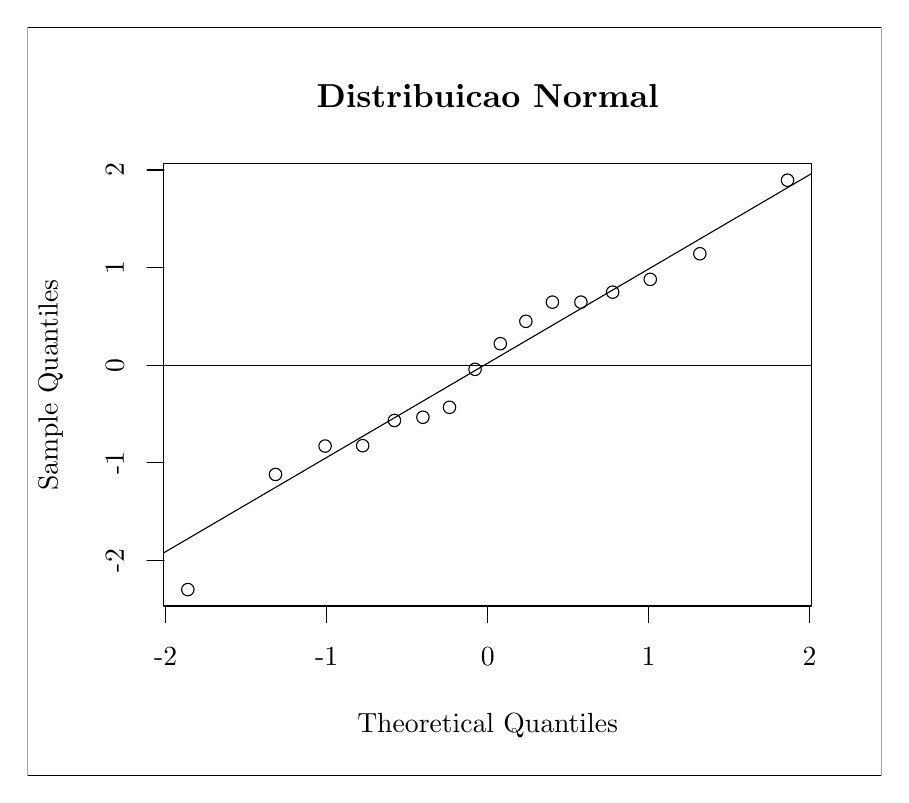
\begin{tikzpicture}[x=1pt,y=1pt]
\definecolor{fillColor}{RGB}{255,255,255}
\path[use as bounding box,fill=fillColor,fill opacity=0.00] (0,0) rectangle (308.44,270.16);
\begin{scope}
\path[clip] ( 49.20, 61.20) rectangle (283.24,220.96);
\definecolor{drawColor}{RGB}{0,0,0}

\path[draw=drawColor,line width= 0.4pt,line join=round,line cap=round] (132.53,128.22) circle (  2.25);

\path[draw=drawColor,line width= 0.4pt,line join=round,line cap=round] (107.47,118.98) circle (  2.25);

\path[draw=drawColor,line width= 0.4pt,line join=round,line cap=round] (170.78,155.96) circle (  2.25);

\path[draw=drawColor,line width= 0.4pt,line join=round,line cap=round] (189.62,170.98) circle (  2.25);

\path[draw=drawColor,line width= 0.4pt,line join=round,line cap=round] (199.91,170.98) circle (  2.25);

\path[draw=drawColor,line width= 0.4pt,line join=round,line cap=round] (161.66,146.71) circle (  2.25);

\path[draw=drawColor,line width= 0.4pt,line join=round,line cap=round] (180.02,164.05) circle (  2.25);

\path[draw=drawColor,line width= 0.4pt,line join=round,line cap=round] (142.82,129.38) circle (  2.25);

\path[draw=drawColor,line width= 0.4pt,line join=round,line cap=round] (242.89,188.46) circle (  2.25);

\path[draw=drawColor,line width= 0.4pt,line join=round,line cap=round] ( 57.87, 67.12) circle (  2.25);

\path[draw=drawColor,line width= 0.4pt,line join=round,line cap=round] (274.57,215.04) circle (  2.25);

\path[draw=drawColor,line width= 0.4pt,line join=round,line cap=round] (152.42,132.99) circle (  2.25);

\path[draw=drawColor,line width= 0.4pt,line join=round,line cap=round] (211.38,174.59) circle (  2.25);

\path[draw=drawColor,line width= 0.4pt,line join=round,line cap=round] (224.97,179.21) circle (  2.25);

\path[draw=drawColor,line width= 0.4pt,line join=round,line cap=round] (121.06,119.12) circle (  2.25);

\path[draw=drawColor,line width= 0.4pt,line join=round,line cap=round] ( 89.55,108.72) circle (  2.25);
\end{scope}
\begin{scope}
\path[clip] (  0.00,  0.00) rectangle (308.44,270.16);
\definecolor{drawColor}{RGB}{0,0,0}

\path[draw=drawColor,line width= 0.4pt,line join=round,line cap=round] ( 49.88, 61.20) -- (282.56, 61.20);

\path[draw=drawColor,line width= 0.4pt,line join=round,line cap=round] ( 49.88, 61.20) -- ( 49.88, 55.20);

\path[draw=drawColor,line width= 0.4pt,line join=round,line cap=round] (108.05, 61.20) -- (108.05, 55.20);

\path[draw=drawColor,line width= 0.4pt,line join=round,line cap=round] (166.22, 61.20) -- (166.22, 55.20);

\path[draw=drawColor,line width= 0.4pt,line join=round,line cap=round] (224.39, 61.20) -- (224.39, 55.20);

\path[draw=drawColor,line width= 0.4pt,line join=round,line cap=round] (282.56, 61.20) -- (282.56, 55.20);

\node[text=drawColor,anchor=base,inner sep=0pt, outer sep=0pt, scale=  1.00] at ( 49.88, 39.60) {-2};

\node[text=drawColor,anchor=base,inner sep=0pt, outer sep=0pt, scale=  1.00] at (108.05, 39.60) {-1};

\node[text=drawColor,anchor=base,inner sep=0pt, outer sep=0pt, scale=  1.00] at (166.22, 39.60) {0};

\node[text=drawColor,anchor=base,inner sep=0pt, outer sep=0pt, scale=  1.00] at (224.39, 39.60) {1};

\node[text=drawColor,anchor=base,inner sep=0pt, outer sep=0pt, scale=  1.00] at (282.56, 39.60) {2};

\path[draw=drawColor,line width= 0.4pt,line join=round,line cap=round] ( 49.20, 77.59) -- ( 49.20,218.72);

\path[draw=drawColor,line width= 0.4pt,line join=round,line cap=round] ( 49.20, 77.59) -- ( 43.20, 77.59);

\path[draw=drawColor,line width= 0.4pt,line join=round,line cap=round] ( 49.20,112.88) -- ( 43.20,112.88);

\path[draw=drawColor,line width= 0.4pt,line join=round,line cap=round] ( 49.20,148.16) -- ( 43.20,148.16);

\path[draw=drawColor,line width= 0.4pt,line join=round,line cap=round] ( 49.20,183.44) -- ( 43.20,183.44);

\path[draw=drawColor,line width= 0.4pt,line join=round,line cap=round] ( 49.20,218.72) -- ( 43.20,218.72);

\node[text=drawColor,rotate= 90.00,anchor=base,inner sep=0pt, outer sep=0pt, scale=  1.00] at ( 34.80, 77.59) {-2};

\node[text=drawColor,rotate= 90.00,anchor=base,inner sep=0pt, outer sep=0pt, scale=  1.00] at ( 34.80,112.88) {-1};

\node[text=drawColor,rotate= 90.00,anchor=base,inner sep=0pt, outer sep=0pt, scale=  1.00] at ( 34.80,148.16) {0};

\node[text=drawColor,rotate= 90.00,anchor=base,inner sep=0pt, outer sep=0pt, scale=  1.00] at ( 34.80,183.44) {1};

\node[text=drawColor,rotate= 90.00,anchor=base,inner sep=0pt, outer sep=0pt, scale=  1.00] at ( 34.80,218.72) {2};

\path[draw=drawColor,line width= 0.4pt,line join=round,line cap=round] ( 49.20, 61.20) --
	(283.24, 61.20) --
	(283.24,220.96) --
	( 49.20,220.96) --
	( 49.20, 61.20);
\end{scope}
\begin{scope}
\path[clip] (  0.00,  0.00) rectangle (308.44,270.16);
\definecolor{drawColor}{RGB}{0,0,0}

\node[text=drawColor,anchor=base,inner sep=0pt, outer sep=0pt, scale=  1.20] at (166.22,241.42) {\bfseries Distribuicao Normal};

\node[text=drawColor,anchor=base,inner sep=0pt, outer sep=0pt, scale=  1.00] at (166.22, 15.60) {Theoretical Quantiles};

\node[text=drawColor,rotate= 90.00,anchor=base,inner sep=0pt, outer sep=0pt, scale=  1.00] at ( 10.80,141.08) {Sample Quantiles};
\end{scope}
\begin{scope}
\path[clip] ( 49.20, 61.20) rectangle (283.24,220.96);
\definecolor{drawColor}{RGB}{0,0,0}

\path[draw=drawColor,line width= 0.4pt,line join=round,line cap=round] ( 49.20, 80.41) -- (283.24,217.42);
\end{scope}
\begin{scope}
\path[clip] (  0.00,  0.00) rectangle (308.44,270.16);
\definecolor{drawColor}{RGB}{0,0,0}

\path[draw=drawColor,line width= 0.4pt,line join=round,line cap=round] ( 49.88, 61.20) -- (282.56, 61.20);

\path[draw=drawColor,line width= 0.4pt,line join=round,line cap=round] ( 49.88, 61.20) -- ( 49.88, 55.20);

\path[draw=drawColor,line width= 0.4pt,line join=round,line cap=round] (108.05, 61.20) -- (108.05, 55.20);

\path[draw=drawColor,line width= 0.4pt,line join=round,line cap=round] (166.22, 61.20) -- (166.22, 55.20);

\path[draw=drawColor,line width= 0.4pt,line join=round,line cap=round] (224.39, 61.20) -- (224.39, 55.20);

\path[draw=drawColor,line width= 0.4pt,line join=round,line cap=round] (282.56, 61.20) -- (282.56, 55.20);

\path[draw=drawColor,line width= 0.4pt,line join=round,line cap=round] ( 49.20, 77.59) -- ( 49.20,218.72);

\path[draw=drawColor,line width= 0.4pt,line join=round,line cap=round] ( 49.20, 77.59) -- ( 43.20, 77.59);

\path[draw=drawColor,line width= 0.4pt,line join=round,line cap=round] ( 49.20,112.88) -- ( 43.20,112.88);

\path[draw=drawColor,line width= 0.4pt,line join=round,line cap=round] ( 49.20,148.16) -- ( 43.20,148.16);

\path[draw=drawColor,line width= 0.4pt,line join=round,line cap=round] ( 49.20,183.44) -- ( 43.20,183.44);

\path[draw=drawColor,line width= 0.4pt,line join=round,line cap=round] ( 49.20,218.72) -- ( 43.20,218.72);
\end{scope}
\begin{scope}
\path[clip] ( 49.20, 61.20) rectangle (283.24,220.96);
\definecolor{drawColor}{RGB}{0,0,0}

\path[draw=drawColor,line width= 0.4pt,line join=round,line cap=round] ( 49.20,148.16) -- (283.24,148.16);
\end{scope}
\begin{scope}
\path[clip] (  0.00,  0.00) rectangle (308.44,270.16);
\definecolor{drawColor}{RGB}{0,0,0}

\path[draw=drawColor,line width= 0.4pt,line join=round,line cap=round] (  0.00,  0.00) --
	(308.44,  0.00) --
	(308.44,270.16) --
	(  0.00,270.16) --
	(  0.00,  0.00);
\end{scope}
\end{tikzpicture}
